\newenvironment{tab}{
  \begin{minipage}{0.1\paperwidth}
    \begin{tabular}{|l|r|r|r|r|}
}{
    \end{tabular}
  \end{minipage}
}
\newenvironment{tree}{
  \begin{minipage}{0.16\paperwidth}
    \begin{tikzpicture}
}{
    \end{tikzpicture}
  \end{minipage}
}
\newcommand\step[1]{
  \framebox[0.4\paperwidth]{#1}
}
\newenvironment{twosteps}{
  % Adjusting the width (by 0cm here) is neede when the margins are too
  % big...
  \begin{adjustwidth}{0cm}{0cm}
}{
  \end{adjustwidth}
}
\newcommand\nop{}

\begin{twosteps}
  \step{
		Etape 1
    \begin{tree}
      \node {-}
      child {node [fill=red!30,label=left:$\to$] {N}
        child {node {O}}
      }
      child {node {S}
        child {node {O}
          child {node {N}}
        }
        child {node {U}}
      };
    \end{tree}
    \begin{tab}
      \hline
      \nop{} & - & O & N\\
      \hline
      -		& 0	& 1 & 2\\
      \hline
      N		& 1	& 1 & 1\\
      \hline
    \end{tab}
  }% \step
  \step {
		Etape 2
    \begin{tree}
      \node {-}
      child {node [fill=red!30] {N}
        child {node [label=left:$\to$] {O}}
      }
      child {node {S}
        child {node {O}
          child {node {N}}
        }
        child {node {U}}
      };
    \end{tree}
    \begin{tab}
      \hline
      \nop{} & - & O & N\\
      \hline
      -		& 0	& 1 & 2\\
      \hline
      N		& 1	& 1 & 1\\
      \hline
      O		& 2	& 1 & 1\\
      \hline
    \end{tab}
  }% \step
\end{twosteps}

\begin{twosteps}
  \step{
		Etape 3
    \begin{tree}
      \node {-}
      child {node {N}
        child {node {O}}
      }
      child {node [fill=red!30,label=left:$\to$] {S}
        child {node {O}
          child {node {N}}
        }
        child {node {U}}
      };
    \end{tree}
    \begin{tab}
      \hline
      \nop{} & - & O & N\\
      \hline
      -		& 0	& 1 & 2\\
      \hline
      S		& 1	& 1 & 2\\
      \hline
    \end{tab}
  }% \step
  \step {
		Etape 4
    \begin{tree}
      \node {-}
      child {node {N}
        child {node {O}}
      }
      child {node [fill=red!30] {S}
        child {node [label=left:$\to$] {O}
          child {node {N}}
        }
        child {node {U}}
      };
    \end{tree}
    \begin{tab}
      \hline
      \nop{} & - & O & N\\
      \hline
      -		& 0	& 1 & 2\\
      \hline
      S		& 1	& 1 & 2\\
      \hline
      O		& 2	& 1 & 2\\
      \hline
    \end{tab}
  }% \step
\end{twosteps}

\begin{twosteps}
  \step {
		Etape 5
    \begin{tree}
      \node {-}
      child {node {N}
        child {node {O}}
      }
      child {node [fill=red!30] {S}
        child {node {O}
          child {node [label=left:$\to$] {N}}
        }
        child {node {U}}
      };
    \end{tree}
    \begin{tab}
      \hline
      \nop{} & - & O & N\\
      \hline
      -		& 0	& 1 & 2\\
      \hline
      S		& 1	& 1 & 2\\
      \hline
      O		& 2	& 1 & 2\\
      \hline
      N		& 3	& 2 & 1\\
      \hline
    \end{tab}
  }% \step
  \step {
		Etape 6
    \begin{tree}
      \node {-}
      child {node {N}
        child {node {O}}
      }
      child {node [fill=red!30] {S}
        child {node {O}
          child {node {N}}
        }
        child {node [label=left:$\to$] {U}}
      };
    \end{tree}
    \begin{tab}
      \hline
      \nop{} & - & O & N\\
      \hline
      -		& 0	& 1 & 2\\
      \hline
      S		& 1	& 1 & 2\\
      \hline
      U		& 2	& 2 & 2\\
      \hline
    \end{tab}
  }% \step
\end{twosteps}
\begin{flushright}
  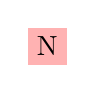
\begin{tikzpicture}
    \node [fill=red!30] {N};
  \end{tikzpicture}
  : \textit{lock} verrouillé\\
  \begin{tikzpicture}
    \node [label=left:$\to$] {N};
  \end{tikzpicture}
  : étape courante
\end{flushright}
\begin{center}
  \textit{Recherche du mot ``on" dans le dictionnaire \{``no", ``son",
    ``su"\}}.
\end{center}
